\section{Sampling and Reconstruction}
\subsection{Introduction}
A typical signal processing system includes 3 stages:
\begin{figure}[h!]
    \centering
    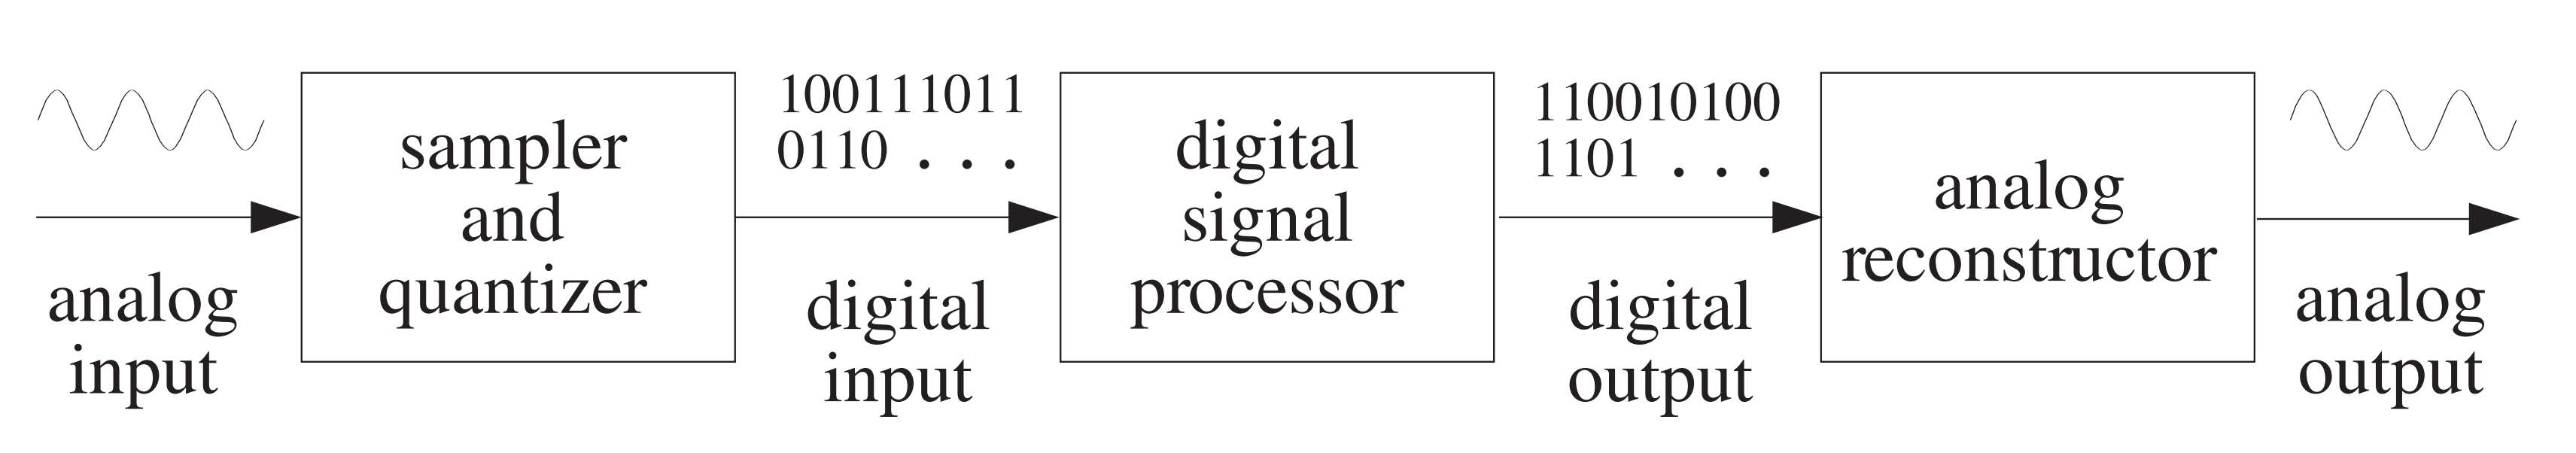
\includegraphics[width=0.6\linewidth]{img/1.png}
\end{figure}

The analog signal is \textbf{\textit{sampled}} and each sample is \textbf{\textit{quantized}} to a finite number of bits (A/D converter).

The digitalized samples are processed by a digital signal processor.
\begin{itemize}
    \item The digital processor can be programmed to perform signal processing operations such as filtering, spectrum estimation.
    \item Digital signal processor can be a general purpose computer, DSP chip or other digital hardware.
\end{itemize}

The resulting output samples are converted back into analog by an \textbf{\textit{analog reconstructor}} (D/A converter).
\subsection{Analog to digital conversion}
Analog to digital (A/D) conversion is a three-step process.
\begin{figure}[h!]
    \centering
    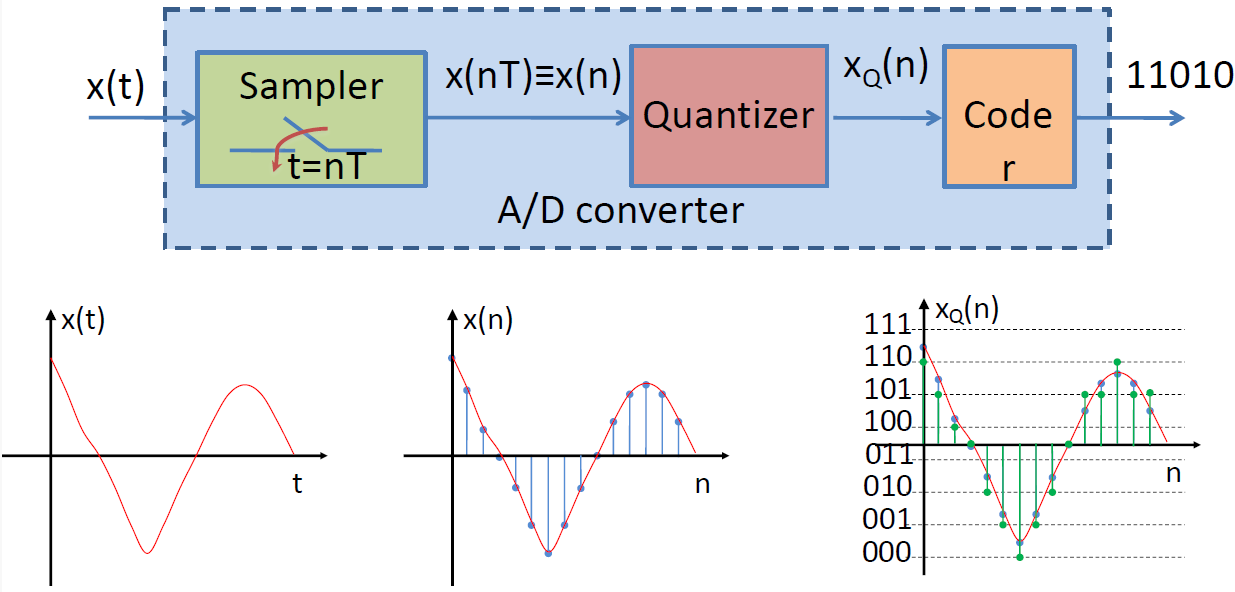
\includegraphics[width=0.7\linewidth]{img/2.png}
    \caption{x(n) is discrete time signal but continus in amplitude}
\end{figure}

* Transform from blue to green is quantizer.
\subsection{Sampling}
Sampling is to convert a continuous time signal into a discrete time signal. The analog signal is periodically measured at every T seconds.
\begin{figure}[h!]
    \centering
    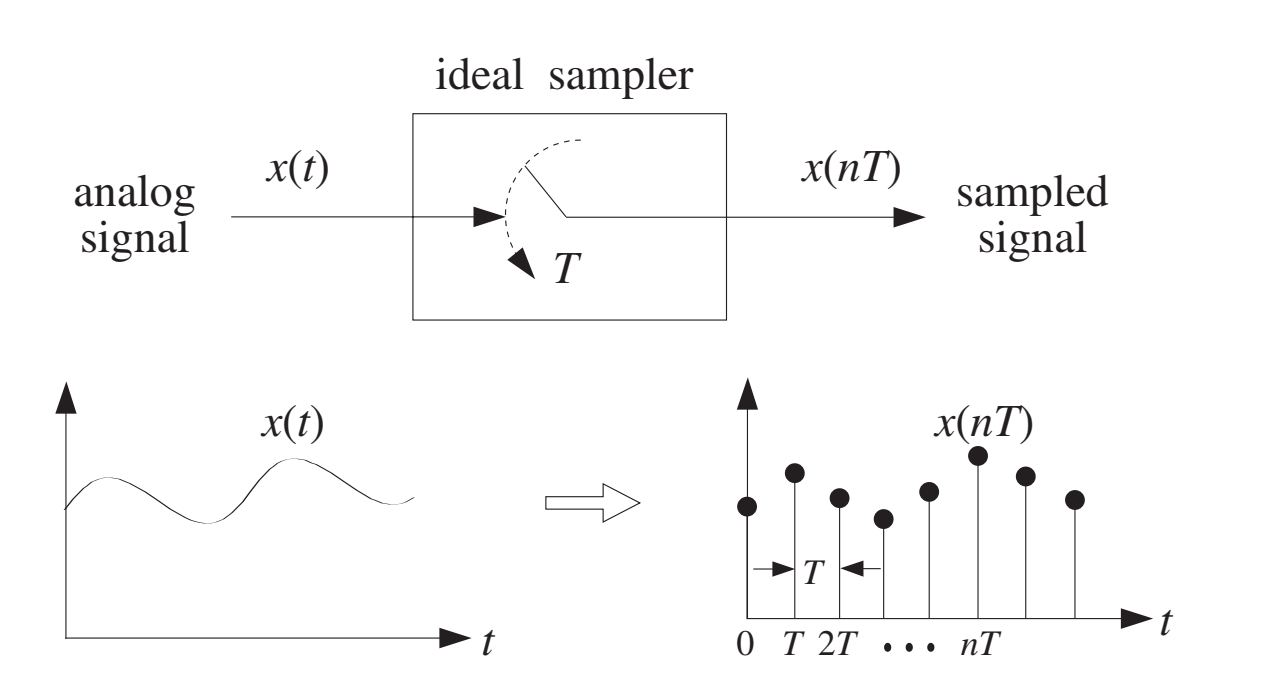
\includegraphics[width=0.5\linewidth]{img/3.png}
\end{figure}
\begin{equation*}
    x(n) \equiv x(nT)=x(t=nT),\ n=…-2, -1, 0, 1, 2, 3…
\end{equation*}
\begin{itemize}
    \item T: sampling interval or sampling period (second);
    \item Fs=1/T: sampling rate or frequency (samples/second or Hz)
\end{itemize}
\subsection{Aliasing of Sinusoids}
In general, the sampling of a continuous-time sinusoidal signal $x(t) = A\cos(2\pi F_0 t + \theta)$ at a sampling rate $ F_s=1/T $ results in a discrete-time signal $x(n)$.

The sinusoids $x_k(t) = A\cos(2\pi F_k t + \theta)$ is sampled at $F_s$, resulting  in a discrete time signal $x_k(n)$.

If $F_k=F_0+kF_s, k=0, \pm 1, \pm 2, ….,$ then $x(n)=x_k(n)$.
\subsection{Spectrum Replication}
\begin{figure}[h!]
    \centering
    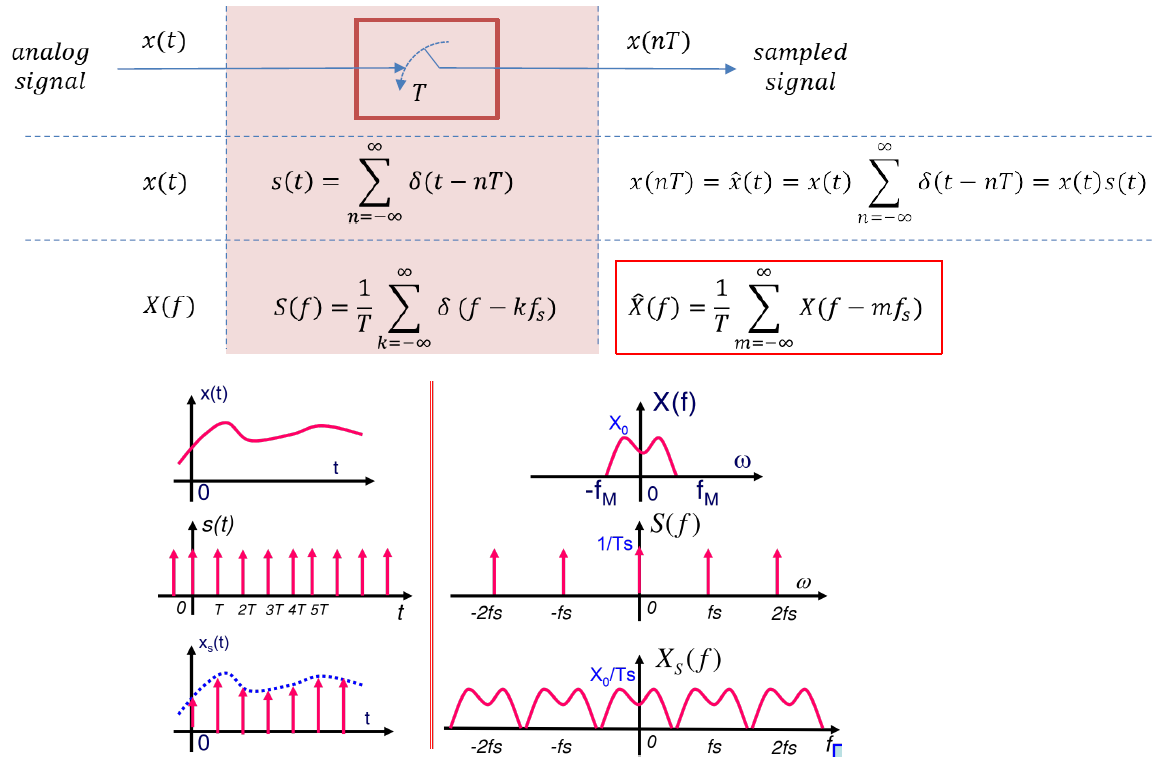
\includegraphics[width=0.7\linewidth]{img/5.png}
\end{figure}

\textbf{Observation}: The spectrum of discrete-time signal is a sum of the original spectrum of analog signal and its periodic replication at the interval $F_s$.
\begin{figure}[h!]
    \centering
    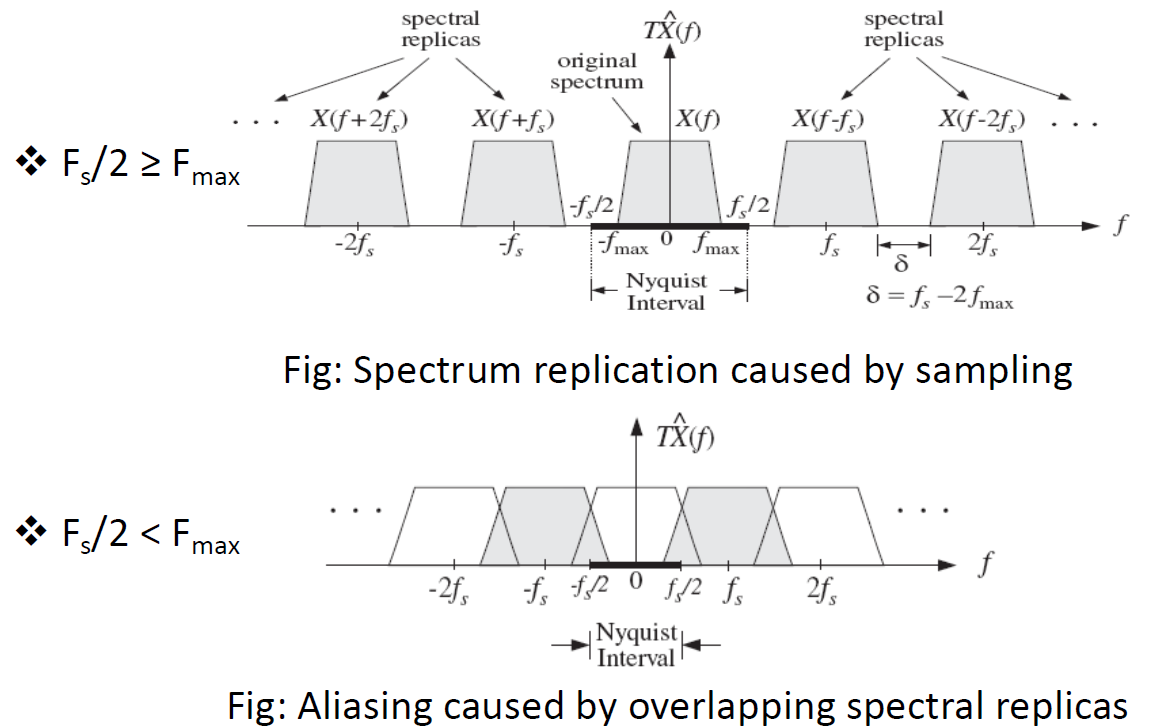
\includegraphics[width=0.7\linewidth]{img/6.png}
\end{figure}
\subsection{Sampling Theorem}
For accurate representation of a signal $x(t)$ by its time samples $x(nT)$, two conditions must be met:
\begin{itemize}
    \item[1)] The signal $x(t)$ must be band-limited, i.e., its frequency spectrum must be limited to $F_{\max}$.
    \item[2)] The sampling rate $F_s$ must be chosen at least twice the maximum frequency $F_{\max}$. $F_s \geq 2F_{\max}$
    \begin{itemize}
        \item $F_s=2F_{\max}$ is called Nyquist rate.
        \item $F_s/2$ is called Nyquist frequency.
        \item $[-F_s/2, F_s/2]$ is Nyquist interval.
    \end{itemize}
\end{itemize}
\begin{figure}[h!]
    \centering
    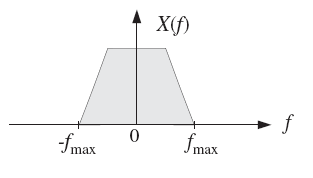
\includegraphics[width=0.3\linewidth]{img/7.png}
    \caption{Typical band-limited spectrum}
\end{figure}
\subsection{Ideal analog reconstruction}
\begin{figure}[h!]
    \centering
    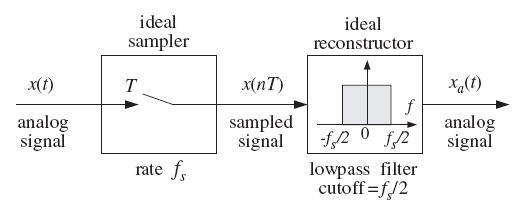
\includegraphics[width=0.5\linewidth]{img/8.png}
    \caption{Ideal reconstructor as a lowpass filter}
\end{figure}
An ideal reconstructor acts as a lowpass filter with cutoff frequency equal to the Nyquist frequency $F_s/2$. An ideal reconstructor (lowpass filter)  $H(F) = \begin{cases}
        T \in [-F_s/2, F_s/2] \\
        0 \qquad otherwise
    \end{cases}$. Then $\widehat{X}_a (F) = \widehat{X}(F) H(F) = X(F)$.
\begin{figure}[h!]
    \centering
    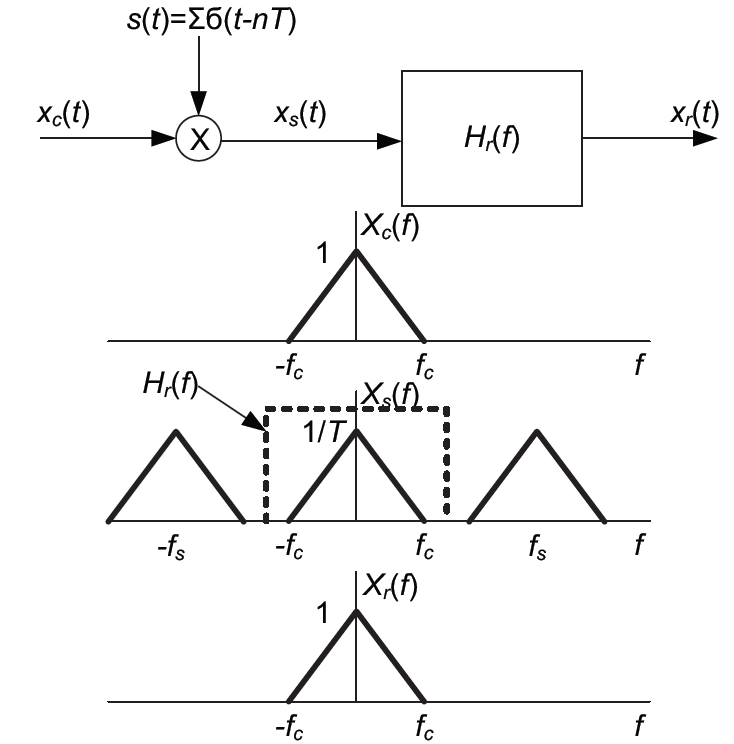
\includegraphics[width=0.35\linewidth]{img/9.png}
    \caption{Example Demonstration}
\end{figure}
\subsection{Ideal antialiasing prefilter}
The signals in practice may not band-limited, thus they must be filtered by a lowpass filter
\begin{figure}[h!]
    \centering
    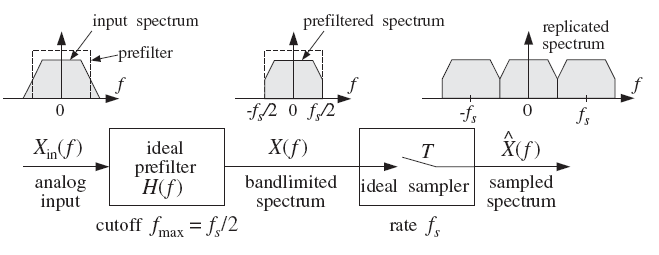
\includegraphics[width=0.6\linewidth]{img/10.png}
    \caption{Ideal antialiasing prefilter}
\end{figure}
\subsection{Practical antialiasing prefilter}
\begin{itemize}
    \item A lowpass filter: Passband $[-F_{pass}, F_{pass}]$ is the frequency range of interest for the application $(F_{max}=F_{pass})$.
    \item The stopband frequency $F_{stop}$ and the minimum stopband attenuation Astop dB must be chosen appropriately to minimize the aliasing effects.
    \item The Nyquist frequency $F_s/2$ is in the middle of transition region.
    \begin{equation*}
        F_s = F_{pass}+F_{stop}
    \end{equation*}
    \item The attenuation of the filter in decibels is defined as (where $f_0$ is a convenient reference frequency, typically taken to be at DC for a lowpass filter):
    \begin{equation*}
        A(F) = -2\log_{10}\left|\dfrac{H(F)}{H(F_0)} \right| \quad (dB)
    \end{equation*}
    \item $\alpha_{10} =A(10F)-A(F)$ (dB/decade): the increase in attenuation when F is changed by a factor of ten.
    \item $\alpha_2 =A(2F)-A(F)$ (dB/octave): the increase in attenuation when F is changed by a factor of two.
\end{itemize}
\begin{figure}[h!]
    \centering
    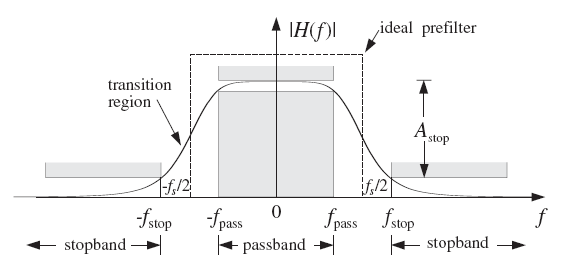
\includegraphics[width=0.5\linewidth]{img/11.png}
\end{figure}




